\section{Phương pháp}

Nghiên cứu này được thiết kế theo hướng nghiên cứu quan sát, hồi cứu kết hợp phân tích trắc lượng thư mục (retrospective, observational, bibliometric study) nhằm phân tích đặc điểm, xu hướng và cấu trúc tri thức của các ấn phẩm thuộc lĩnh vực KKhoa học Thông tin và Thư viện bị thu hồi trong giai đoạn 2021 - 2026. Quy trình thực hiện và báo cáo nghiên cứu được xây dựng dựa trên các khuyến nghị của PRIBA (Preferred Reporting Items for Bibliometric Analysis), nhằm chuẩn hóa và tăng cường tính minh bạch trong báo cáo nghiên cứu trắc lượng thư mục dựa trên cấu trúc tham chiếu từ PRISMA checklist. PRIBA được áp dụng xuyên suốt nghiên cứu, từ xác định mục tiêu, nguồn dữ liệu, tiêu chí lựa chọn, chiến lược tìm kiếm, chỉ số và công cụ phân tích đến trình bày kết quả, thảo luận, hạn chế và các thông tin về hỗ trợ nghiên cứu, xung đột lợi ích và khả năng truy cập dữ liệu.

\subsection{Dữ liệu gốc}

Nghiên cứu sử dụng dữ liệu từ ba nguồn chính gồm Scopus, Web of Science (WoS) và Retraction Watch Database (RWD, \url{https://gitlab.com/crossref/retraction-watch-data}) nhằm kết hợp thông tin thư mục của các ấn phẩm với thông tin chi tiết về các sự kiện thu hồi. Cách tiếp cận đa nguồn này cho phép tận dụng thế mạnh của từng cơ sở dữ liệu: Scopus và WoS chủ yếu cung cấp các thuộc tính thư mục của ấn phẩm, trong khi RWD cung cấp thông tin chuyên biệt về tình trạng, thời điểm và lý do thu hồi.

Dữ liệu thư mục được thu thập từ Scopus và WoS bằng bộ từ khóa được xây dựng theo chủ đề nghiên cứu, với phạm vi thời gian từ năm 2021 đến tháng 7 năm 2026 \textbf{[mô tả cụ thể bộ lọc và tiêu chí truy vấn được áp dụng trên Scopus/WoS]}. Việc lựa chọn giai đoạn này nhằm tập trung vào các xu hướng xuất bản và những vấn đề liên quan đến tính toàn vẹn học thuật trong giai đoạn hậu đại dịch COVID-19. Tổng cộng 583 bản ghi được thu thập từ Scopus và WoS trước các bước xử lý và hợp nhất dữ liệu.

Đối với thông tin về các sự kiện thu hồi, nghiên cứu sử dụng Retraction Watch Database (RWD), một cơ sở dữ liệu chuyên biệt về các ấn phẩm bị thu hồi. Tập dữ liệu RWD được tải xuống đầy đủ vào ngày 31/07/2026, bao gồm 65.898 bản ghi tại thời điểm thu thập. RWD được lựa chọn vì có phạm vi bao phủ rộng và cung cấp nhiều trường dữ liệu chuyên biệt liên quan đến các sự kiện thu hồi, bao gồm các trường như ngày thu hồi và lý do thu hồi. Bên cạnh đó, RWD đã được sử dụng rộng rãi trong các nghiên cứu về thu hồi ấn phẩm và trắc lượng thư mục \textbf{[liệt kê danh sách các bài viết]}. Để bảo đảm tập dữ liệu chỉ phản ánh các sự kiện thu hồi chính thức, RWD và các nguồn dữ liệu liên quan được lọc thô với điều kiện: Chỉ các bản ghi có trạng thái \textit{Retraction} (thu hồi chính thức) được giữ lại; các loại thông báo khác như \textit{Correction} (đính chính), \textit{Expression of Concern} (tuyên bố quan ngại) và \textit{Reinstatement} (khôi phục bài báo) được loại bỏ. Tiêu chí này nhằm phân biệt rõ sự kiện thu hồi thực sự với các hình thức điều chỉnh, cảnh báo hoặc khôi phục ấn phẩm, qua đó bảo đảm rằng dữ liệu đầu vào phản ánh đúng đối tượng nghiên cứu.

Cần lưu ý rằng RWD chỉ ghi nhận những trường hợp thu hồi đã được điều tra và công khai bởi các tạp chí hoặc nhà xuất bản. Do đó, tập dữ liệu phản ánh các trường hợp thu hồi đã được phát hiện, điều tra và ghi nhận trong phạm vi bao phủ của RWD, chứ không đại diện cho toàn bộ các hoạt động thu hồi sau này trong thực tế. Vì vậy, các kết quả nghiên cứu cần được diễn giải trong phạm vi các trường hợp đã được báo cáo và ghi nhận trong cơ sở dữ liệu mà chúng tôi đã thu thập vào thời gian trên.

Quy trình sàng lọc tài liệu được xây dựng dựa trên bốn tiêu chí chính (EC1 - EC4), như được minh họa trong hình \figref{fig:eligibility-criteria}. EC1 thiết lập khung thời gian xuất bản, giới hạn kết quả ở các nghiên cứu được công bố từ năm 2021 đến 2026. EC2 quy định về ngôn ngữ, chỉ bao gồm các tài liệu được viết bằng tiếng Anh. EC3 tập trung vào lĩnh vực chủ đề, hướng đến các nghiên cứu thuộc ngành Khoa học Thông tin và Thư viện (LIS) thông qua việc tìm kiếm trong các trường Tiêu đề, Từ khóa và Tóm tắt bằng chuỗi từ khóa chuyên ngành LIS cốt lõi. Cuối cùng, EC4 loại bỏ dữ liệu không hợp lệ bằng cách xác định và lọc ra các tài liệu đã bị thu hồi được dán nhãn là \textit{Retracted Publication}, \textit{Retracted} hoặc \textit{Retraction}.

\begin{figure}[H]
    \centering
    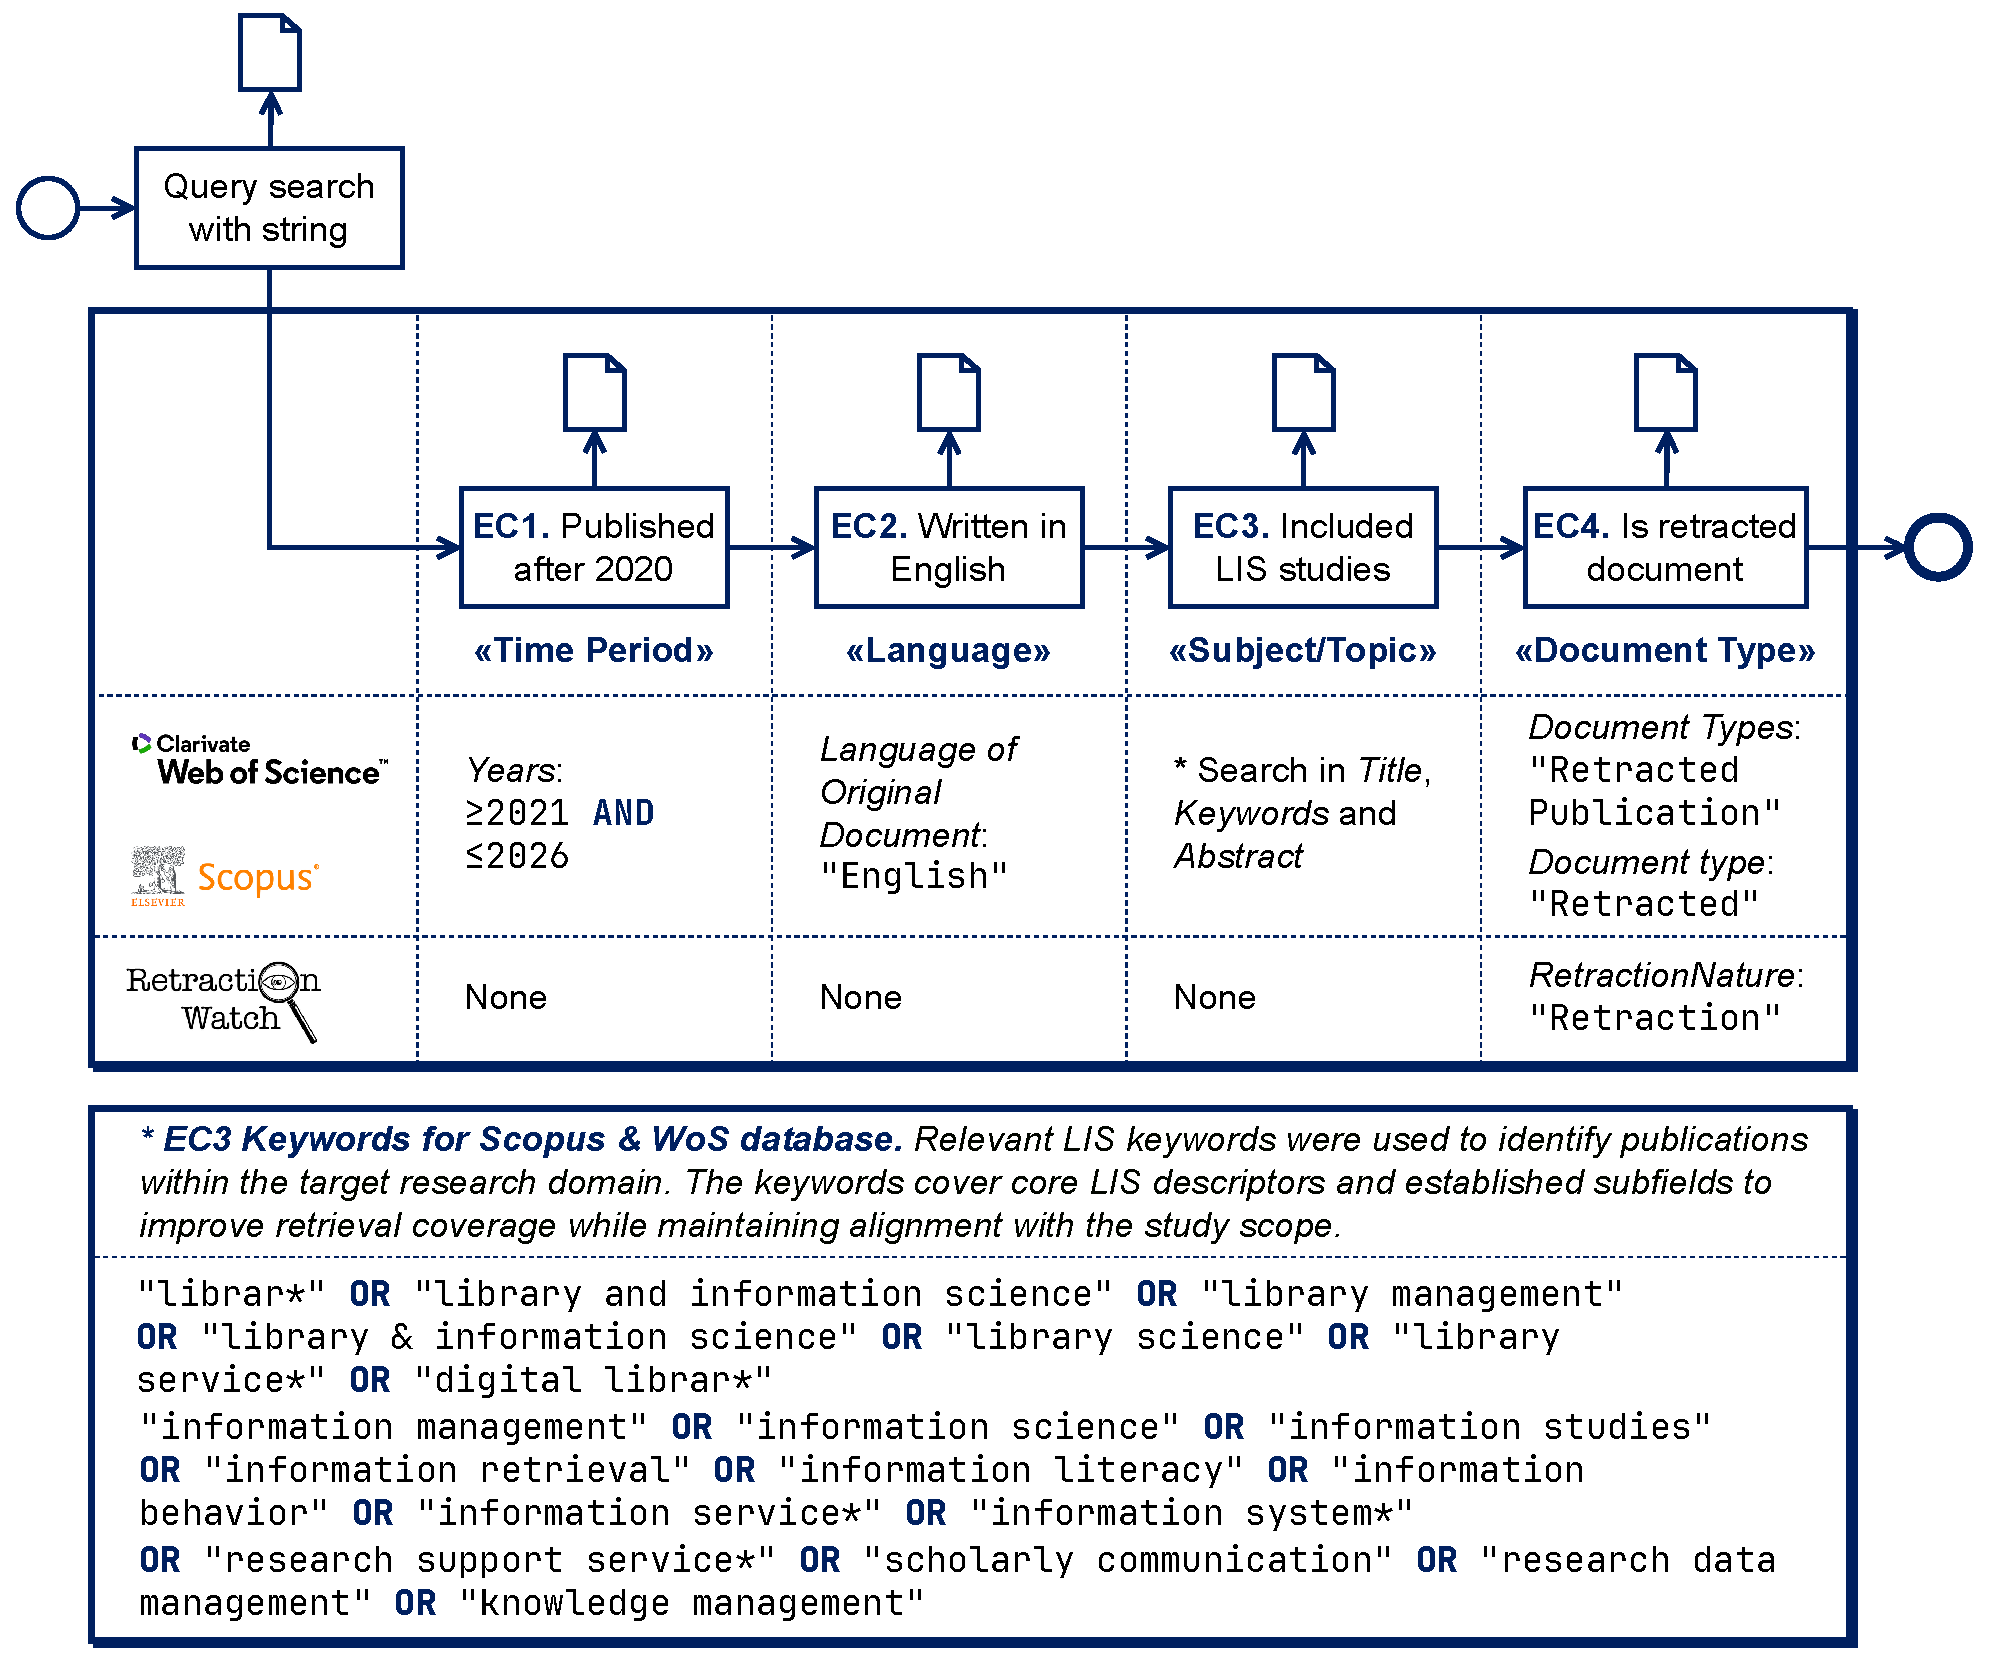
\includegraphics[width=\textwidth]{figures/methods/eligibility-criteria.pdf}
    \caption{Sơ đồ quy trình sàng lọc tài liệu và các tiêu chí lựa chọn (EC1 - EC4)}
    \label{fig:eligibility-criteria}
\end{figure}

\subsection{Chỉ số trắc lượng thư mục}

Việc lựa chọn các chỉ số trắc lượng thư mục được thực hiện nhằm phản ánh ba khía cạnh chính của các ấn phẩm Khoa học Thông tin và Thư viện bị thu hồi trong giai đoạn 2021--2026, bao gồm quy mô thu hồi, mức độ hợp tác giữa các tác giả và đặc điểm của hợp tác trong nước và quốc tế. Trên cơ sở đó, nghiên cứu sử dụng ba nhóm chỉ số gồm số lượng ấn phẩm bị thu hồi (Retraction Count), Chỉ số Hợp tác trong nước (Domestic Collaboration Index -- DCI) và Chỉ số Hợp tác quốc tế (International Collaboration Index -- ICI), kết hợp với Tỷ số DCI/ICI và Hồ sơ hợp tác trong nước.

Số lượng ấn phẩm bị thu hồi được sử dụng làm chỉ số cơ bản để mô tả quy mô và sự biến động của hiện tượng thu hồi theo thời gian, quốc gia, tạp chí hoặc các nhóm phân tích khác. Đây là chỉ số trực tiếp và dễ diễn giải, cho phép xác định những năm, quốc gia hoặc nhóm đối tượng có số lượng ấn phẩm bị thu hồi cao hơn. Trong nghiên cứu này, Retraction Count đóng vai trò là thước đo nền tảng để nhận diện các pattern chính trong dữ liệu trước khi tiến hành phân tích sâu hơn về đặc điểm hợp tác. Tuy nhiên, số lượng tuyệt đối không phản ánh trực tiếp cường độ hay cấu trúc hợp tác và có thể chịu ảnh hưởng bởi quy mô xuất bản hoặc các sự kiện thu hồi hàng loạt. Vì vậy, chỉ số này được sử dụng chủ yếu để mô tả quy mô và xu hướng, thay vì được diễn giải như một thước đo độc lập về mức độ rủi ro hoặc chất lượng nghiên cứu.

Để phân tích mô hình hợp tác, nghiên cứu sử dụng DCI và ICI, được xây dựng dựa trên cách tiếp cận của Garg và Padhi. Hai chỉ số này được lựa chọn vì cho phép đánh giá mức độ tham gia tương đối của hợp tác trong nước và hợp tác quốc tế so với mức trung bình của toàn bộ tập hợp nghiên cứu. Khác với số lượng hợp tác tuyệt đối, DCI và ICI có tính đến quy mô xuất bản và do đó phù hợp hơn để so sánh các đơn vị có mức độ sản xuất học thuật khác nhau. Trong bối cảnh nghiên cứu về các ấn phẩm bị thu hồi, việc sử dụng hai chỉ số này giúp xác định liệu một quốc gia hoặc nhóm đối tượng có xu hướng tham gia vào hợp tác trong nước hoặc quốc tế với mức độ cao hơn hay thấp hơn mức trung bình quan sát được trong toàn bộ tập dữ liệu.

Chỉ số Hợp tác trong nước (DCI) được sử dụng để đánh giá mức độ hợp tác giữa các tác giả thuộc cùng một quốc gia. Chỉ số được tính theo công thức:
\begin{equation}
DCI = \frac{D_i / D_{io}}{D_o / D_{oo}} \times 100
\end{equation}
Trong đó, $D_i$ là số ấn phẩm có hợp tác trong nước của một quốc gia trong khoảng thời gian nghiên cứu; $D_{io}$ là tổng số ấn phẩm của quốc gia đó trong cùng khoảng thời gian; $D_o$ là tổng số ấn phẩm hợp tác trong nước của toàn bộ tập dữ liệu; và $D_{oo}$ là tổng số ấn phẩm của toàn bộ tập dữ liệu. Giá trị $\text{DCI} = 100$ cho thấy mức độ hợp tác trong nước của quốc gia tương đương với mức trung bình của toàn bộ tập dữ liệu; $\text{DCI} > 100$ cho thấy mức độ hợp tác trong nước cao hơn mức trung bình; trong khi $\text{DCI} < 100$ cho thấy mức độ thấp hơn mức trung bình.

Tương tự, Chỉ số Hợp tác quốc tế (ICI) được sử dụng để đánh giá mức độ tham gia của một quốc gia vào các ấn phẩm có sự hợp tác giữa các quốc gia. Chỉ số được tính theo công thức:
\begin{equation}
ICI = \frac{I_i / I_{io}}{I_o / I_{oo}} \times 100
\end{equation}
Trong đó, $I_i$ là số ấn phẩm hợp tác quốc tế của quốc gia trong khoảng thời gian nghiên cứu; $I_{io}$ là tổng số ấn phẩm của quốc gia đó; $I_o$ là tổng số ấn phẩm hợp tác quốc tế của toàn bộ tập dữ liệu; và $I_{oo}$ là tổng số ấn phẩm của toàn bộ tập dữ liệu. Tương tự DCI, $\text{ICI} = 100$ biểu thị mức độ hợp tác quốc tế tương đương với mức trung bình; $\text{ICI} > 100$ biểu thị mức độ cao hơn mức trung bình; và $\text{ICI} < 100$ biểu thị mức độ thấp hơn mức trung bình. Việc kết hợp DCI và ICI cho phép phân biệt rõ hơn giữa xu hướng hợp tác trong nước và hợp tác quốc tế thay vì chỉ dựa trên tổng số ấn phẩm hợp tác.

Bên cạnh hai chỉ số riêng biệt, Tỷ số DCI/ICI được sử dụng để đánh giá tương quan tương đối giữa xu hướng hợp tác trong nước và hợp tác quốc tế của từng quốc gia. Chỉ số này được tính bằng tỷ số giữa DCI và ICI. Giá trị $\text{DCI/ICI} > 1$ cho thấy mức độ hợp tác trong nước tương đối nổi trội hơn hợp tác quốc tế, trong khi $\text{DCI/ICI} < 1$ cho thấy hợp tác quốc tế tương đối nổi trội hơn. Giá trị xấp xỉ 1 cho thấy hai hình thức hợp tác có mức độ tương đối tương đồng. Việc sử dụng tỷ số này giúp bổ sung cho DCI và ICI bằng một thước đo tổng hợp, qua đó thuận tiện hơn trong việc xác định định hướng hợp tác chủ đạo của từng quốc gia. Tuy nhiên, tỷ số này được diễn giải như một chỉ báo tương đối về cấu trúc hợp tác, không phải là tỷ lệ phần trăm ấn phẩm hợp tác trong nước so với hợp tác quốc tế.

\subsection{Quy trình phân tích}

Nhằm đảm bảo độ tin cậy, tính minh bạch và khả năng tái lập của tập dữ liệu phân tích, nghiên cứu này áp dụng khung đảm bảo chất lượng dữ liệu dựa trên VALOR trong quá trình tiền xử lý và tích hợp dữ liệu đa nguồn. Khung này được điều chỉnh phù hợp với đặc điểm của nghiên cứu trắc lượng thư mục về các ấn phẩm bị thu hồi, tập trung vào năm khía cạnh chính: \textit{(i) kiểm chứng tính nhất quán dữ liệu; (ii) đồng bộ hóa khoảng thời gian; (iii) ghi chép tài liệu; (iv) xác thực kết quả phân tích; (v) đảm bảo khả năng tái lập} \parencite{hoang2025}. Các yêu cầu và cách thức triển khai cụ thể của khung VALOR được điều chỉnh cho nghiên cứu này được trình bày tại Bảng~\tableref{table:valor-framework}.

\begin{table}[H]
\centering
\caption{Khung VALOR được điều chỉnh để kiểm soát chất lượng trong nghiên cứu trắc lượng thư mục đa nguồn về các ấn phẩm bị thu hồi}
\label{table:valor-framework}
\begin{tabularx}{\textwidth}{>{\raggedright\arraybackslash}p{1.5in} >{\raggedright\arraybackslash}X}
\toprule
\textbf{Khía cạnh} & \textbf{Yêu cầu và nội dung xem xét được điều chỉnh cho nghiên cứu} \\
\midrule
Kiểm chứng tính nhất quán của dữ liệu & 
\begin{itemize}[label=\ding{109}, leftmargin=*, wide, nosep, before=\vspace{-11pt}]
    \item Kiểm tra và chuẩn hóa cấu trúc, tên trường và kiểu dữ liệu giữa Scopus/WoS và RWD.
    \item Kiểm tra tính nhất quán của DOI trong các cơ sở dữ liệu.
    \item Kiểm tra quan hệ giữa tác giả, mã tác giả và đơn vị công tác trong cơ sở dữ liệu.
    \item Chuẩn hóa thông tin nhà xuất bản và tạp chí.
    \item Kiểm tra và xử lý ngày xuất bản và ngày thu hồi để tính thời gian thu hồi ấn phẩm.
    \item Chuẩn hóa và phân loại các nhãn nguyên nhân thu hồi.
\end{itemize} \\
\addlinespace
Căn chỉnh phạm vi thời gian & 
\begin{itemize}[label=\ding{109}, leftmargin=*, wide, nosep, before=\vspace{-10pt}]
    \item Đồng nhất phạm vi nghiên cứu 2021 - 2026 giữa các nguồn.
    \item Kiểm tra sự khác biệt giữa ngày xuất bản gốc và ngày thu hồi.
    \item Chuẩn hóa định dạng ngày và xác định cách tính thời gian thu hồi ấn phẩm.
    \item Ghi nhận thời điểm truy xuất dữ liệu từ từng nguồn nhằm kiểm soát khác biệt do tần suất cập nhật cơ sở dữ liệu.
\end{itemize} \\
\addlinespace
Ghi nhận và lập tài liệu & 
\begin{itemize}[label=\ding{109}, leftmargin=*, wide, nosep, before=\vspace{-10pt}]
    \item Ghi nhận chiến lược/câu lệnh tìm kiếm cho từng cơ sở dữ liệu.
    \item Ghi lại các bước lập hồ sơ dữ liệu, trích xuất biến, chuẩn hóa, xử lý giá trị thiếu và khử trùng lặp cho từng nguồn.
    \item Ghi nhận quy tắc xử lý DOI trùng và trường hợp một bài báo có nhiều bản ghi thu hồi.
    \item Ghi nhận quy trình tích hợp Scopus/WoS với RWD bằng DOI.
    \item Ghi nhận quy tắc gom nhóm nguyên nhân thu hồi.
\end{itemize} \\
\addlinespace
Xác thực kết quả phân tích & 
\begin{itemize}[label=\ding{109}, leftmargin=*, wide, nosep, before=\vspace{-10pt}]
    \item Đối chiếu số lượng bản ghi trước và sau từng bước xử lý.
    \item Kiểm tra tính nhất quán của số lượng bài thu hồi theo năm, tạp chí, nhà xuất bản và nguyên nhân.
    \item Kiểm tra tính hợp lệ của các chỉ số trắc lượng thư mục, cách tính thời gian thu hồi ấn phẩm và các thống kê mô tả.
    \item Đối chiếu các bảng kết quả và biểu đồ với dữ liệu nguồn.
\end{itemize} \\
\addlinespace
Khả năng tái lập & 
\begin{itemize}[label=\ding{109}, leftmargin=*, wide, nosep, before=\vspace{-10pt}]
    \item Lưu trữ dữ liệu và kết quả xử lý dưới định dạng Parquet.
    \item Cung cấp mã nguồn và quy trình xử lý bằng Python/SQL.
    \item Ghi nhận phiên bản Python, DuckDB và công cụ thực thi code (Google Colab).
    \item Mô tả toàn bộ quy trình từ thu thập dữ liệu $\rightarrow$ tiền xử lý $\rightarrow$ phân tích.
    \item Ghi nhận quy tắc xử lý có thể ảnh hưởng đến kết quả phân tích.
\end{itemize} \\
\bottomrule
\end{tabularx}
\end{table}

Toàn bộ quy trình thu thập, làm sạch, chuẩn hóa, tích hợp và phân tích dữ liệu được triển khai bằng ngôn ngữ lập trình \textbf{Python} phiên bản 3.12.13 trên nền tảng \textbf{Google Colab} (minh họa tại Hình~\figref{fig:database-pipeline}), qua đó hỗ trợ tự động hóa quy trình xử lý dữ liệu, quản lý mã nguồn phân tích và duy trì khả năng tái thực hiện các bước phân tích đối với tập dữ liệu các ấn phẩm bị thu hồi trong giai đoạn 2021 - 2026.

\begin{figure}[H]
    \centering
    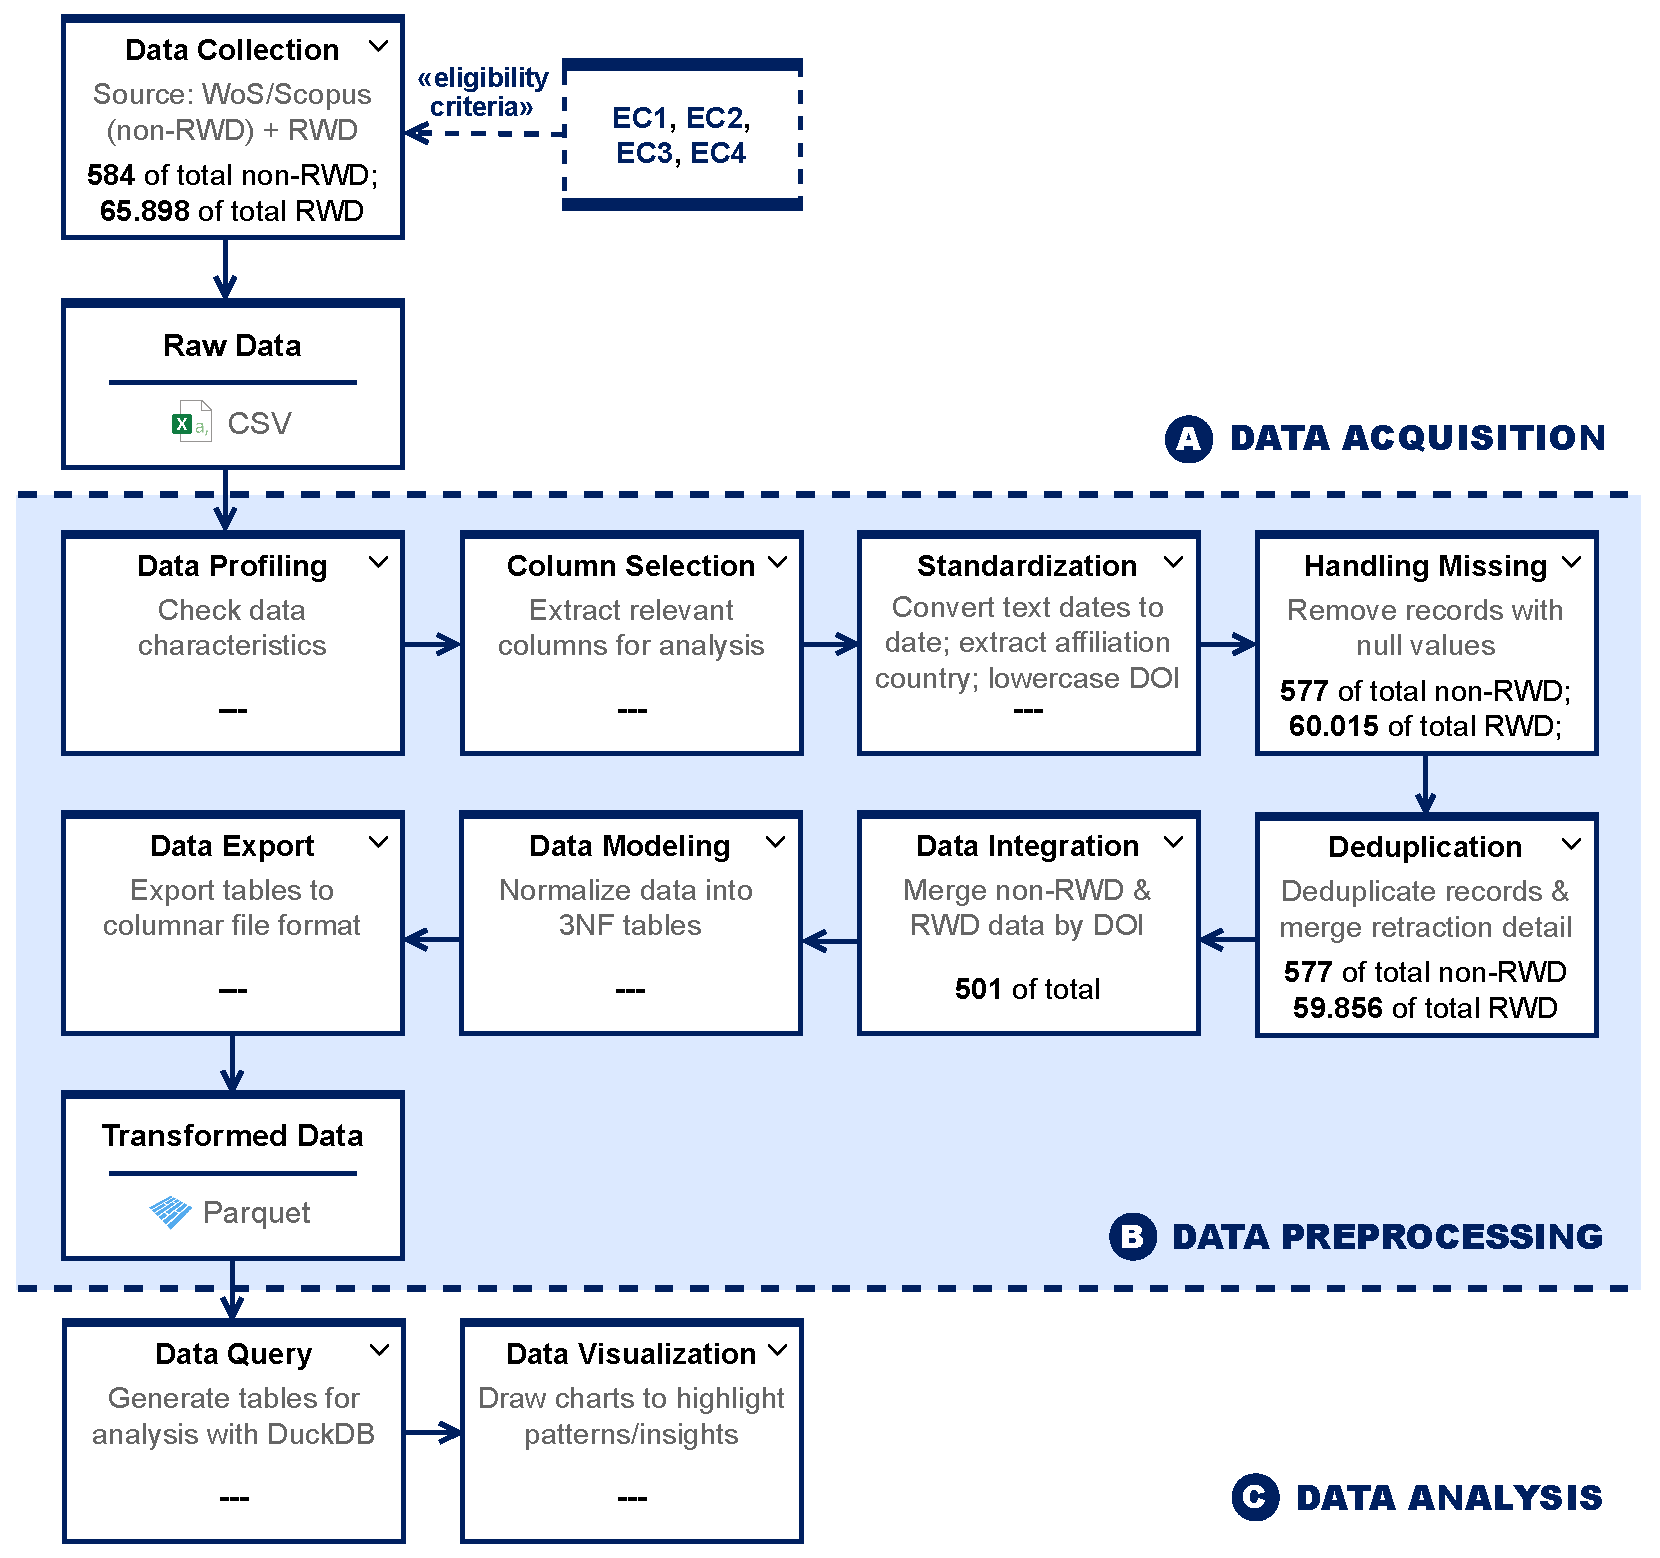
\includegraphics[width=\textwidth]{figures/methods/data-pipeline.pdf}
    \caption{Quy trình từ lúc thu thập đến phân tích dữ liệu nghiên cứu}
    \label{fig:database-pipeline}
\end{figure}

Sử dụng khung VALOR, nhóm nghiên cứu triển khai theo nguyên tắc tiến hành lập hồ sơ dữ liệu trước, xử lý dữ liệu sau, trong đó các đặc điểm và sự không thống nhất trong dữ liệu được phát hiện từ từng nguồn dữ liệu được sử dụng để xác định các bước tiền xử lý tương ứng.

Đối với Scopus và WoS, hồ sơ dữ liệu cho thấy các trường thông tin tác giả (mã ID, tên và địa chỉ công tác) được phân tách bằng dấu chấm phẩy (;) và ánh xạ theo vị trí với số lượng giá trị tương ứng với số lượng tác giả và cho phép lặp lại khi nhiều tác giả có cùng thông tin. Trường địa chỉ công tác chứa đồng thời tên tác giả, cơ quan, địa chỉ và quốc gia, trong khi tên nhà xuất bản và tạp chí (Source title) được viết hoàn toàn bằng chữ thường. Đối với RWD, DOI có định dạng tương ứng và có thể sử dụng làm khóa liên kết với Scopus/WoS. Tuy nhiên, thông tin tác giả với quốc gia công tác không duy trì được quan hệ tương ứng do các quốc gia trùng nhau được gộp thành danh sách duy nhất. Tên nhà xuất bản và tạp chí trong RWD đã được chuẩn hóa cách viết hoa. Do đó, các trường tác giả của Scopus/WoS được giữ cấu trúc phân tách để bảo toàn ánh xạ; địa chỉ công tác được chuẩn hóa và trích xuất quốc gia; thông tin quốc gia công tác từ RWD được loại khỏi phân tích; DOI được chuẩn hóa để liên kết các nguồn; và tên nhà xuất bản, tạp chí của Scopus/WoS được loại bỏ, ưu tiên sử dụng các trường tương ứng từ RWD.

Trên cơ sở lập hồ sơ dữ liệu, các biến cốt lõi được trích xuất theo mục tiêu phân tích: Scopus/WoS giữ DOI, thông tin tác giả, mã định danh và đơn vị công tác để phân tích đặc điểm và mạng lưới hợp tác; RWD giữ DOI, tạp chí, nhà xuất bản, thời gian xuất bản, thời gian thu hồi và nguyên nhân thu hồi để phân tích đặc điểm và xu hướng thu hồi. Bước này giúp giảm dữ liệu dư thừa và tập trung các bước xử lý tiếp theo vào không gian biến phục vụ trực tiếp cho phân tích.


Sau khi trích xuất các trường dữ liệu cốt lõi, dữ liệu được tiếp tục làm sạch và xử lý giá trị thiếu. Đối với Scopus và WoS, việc kiểm tra các trường định 2 bản ghi thiếu tên tác giả, 7 bản ghi thiếu mã định danh tác giả, 1 bản ghi thiếu DOI và 2 bản ghi thiếu đơn vị công tác. Sau khi loại bỏ các bản ghi không đáp ứng yêu cầu, 577/584 bản ghi được giữ lại. Đối với RWD, 2.519 bản ghi thiếu DOI và 3.365 bản ghi có DOI ở trạng thái ``Unavailable'', do đó 5.884 bản ghi được loại bỏ, còn 60.015/65.899 bản ghi. Theo \cite{retractionwatch_appendix_a}, giá trị ``Unavailable'' hoặc trường trống cho biết DOI không được xác định tại thời điểm bản ghi được đưa vào cơ sở dữ liệu; vì vậy, các bản ghi này được loại bỏ để đảm bảo DOI có thể được sử dụng làm khóa định danh và liên kết dữ liệu đa nguồn.

Ở bước khử trùng lặp, không phát hiện bản ghi trùng lặp trong Scopus và WoS, trong khi RWD còn 59.856 bản ghi sau khi xử lý các trường hợp bản ghi trùng lặp và trùng thông tin DOI. Khi một DOI xuất hiện trong nhiều bản ghi thu hồi, các bản ghi được hợp nhất với iteue chí: nếu cùng ngày, giữ nguyên ngày thu hồi và gộp các lý do; nếu khác ngày, chọn ngày thu hồi sớm nhất và hợp nhất toàn bộ lý do. Cách xử lý này đảm bảo mỗi ấn phẩm chỉ được tính một lần, đồng thời phản ánh đúng khoảng thời gian thực tế mà một bài báo sai phạm tồn tại trước khi bị phát hiện và từ đó làm mốc tính thời gian thu hồi ấn phẩm.

Sau khi làm sạch và chuẩn hóa riêng từng nguồn, dữ liệu Scopus, WoS và RWD được tích hợp thành một tập dữ liệu thống nhất sử dụng mã DOI làm khóa liên kết chính. Hai bản ghi từ hai nguồn được ghép khi có cùng DOI; các bản ghi không tìm thấy DOI tương ứng ở nguồn còn lại được loại khỏi tập dữ liệu tích hợp. Việc sử dụng DOI giúp hạn chế sai lệch do khác biệt về định dạng hoặc siêu dữ liệu giữa các nguồn, đồng thời tránh rủi ro ghép sai hoặc bỏ sót khi đối sánh dựa trên tiêu đề hay tên tác giả. Kết quả là 492 bản ghi được đối soát và tích hợp vào tập dữ liệu chung, bảo đảm tính nhất quán và độ bao phủ của dữ liệu phân tích.

Để chuẩn hóa và hệ thống hóa các nhãn nguyên nhân thu hồi từ CSDL RWD, nghiên cứu xây dựng các nhóm nguyên nhân chính dựa trên cơ sở tham khảo và đối chiếu với hệ thống phân loại được sử dụng trong các nghiên cứu trước đây \parencite{tiwari2026, okyay2025}. Các nhãn nguyên nhân ban đầu sau đó được ánh xạ vào một trường phân loại mới, {\sffamily reason\_category}, nhằm thống nhất cách biểu diễn và tạo cơ sở cho các phân tích tiếp theo. Hệ thống phân loại và nguyên tắc ánh xạ cụ thể được trình bày tại Bảng~\tableref{tab:reason_category}.

\begin{table}[H]
\centering
\caption{Phân loại nguyên nhân thu hồi vào từng nhóm}
\label{tab:reason_category}
\small
\begin{tabularx}{\textwidth}{>{\hsize=0.28\hsize\raggedright\arraybackslash}X >{\hsize=1.72\hsize\raggedright\arraybackslash}X}
\toprule
\textbf{Nhóm} & \textbf{Nguyên nhân cụ thể} \\
\midrule
Authorship issues & Breach of Policy by Author; Concerns/Issues about Authorship/Affiliation; Conflict of Interest; False/Forged Authorship; Objections by Author(s) \\
\addlinespace
Data concerns & Concerns/Issues about Article; Concerns/Issues about Data; Concerns/Issues about Image; Concerns/Issues about Results and/or Conclusions; Unreliable Data; Unreliable Image; Unreliable Results and/or Conclusions \\
\addlinespace
Duplication & Duplication of/in Article \\
\addlinespace
Error & Error by Journal/Publisher; Error in Data \\
\addlinespace
Ethical issues & Concerns/Issues about Human Subject Welfare; Informed/Patient Consent - None/Withdrawn; Lack of IRB/IACUC Approval and/or Compliance \\
\addlinespace
Fraud & Paper Mill; Rogue Editor \\
\addlinespace
Legal issues & Concerns/Issues about Third Party Involvement; Investigation by Company/Institution; Investigation by Journal/Publisher; Investigation by Third Party; Objections by Third Party \\
\addlinespace
Peer review issues & Compromised Peer Review; Concerns/Issues about Peer Review \\
\addlinespace
Plagiarism & Plagiarism of/in Article; Taken from Dissertation/Thesis \\
\addlinespace
Randomly generated content & Computer-Aided Content or Computer-Generated Content \\
\addlinespace
Referencing issues & Concerns/Issues about Referencing/Attributions \\
\addlinespace
Transparency issues & Author Unresponsive; Original Data and/or Images not Provided and/or not Available \\
\addlinespace
Others & \\
\bottomrule
\end{tabularx}
\end{table}

{\noindent\robotocondensed\footnotesize IRB = Institutional Review Board, IACUC = Institutional Animal Care and Use Committee.}

\vspace{6pt}

Sau khi tích hợp và làm sạch, dữ liệu được chuyển sang mô hình cơ sở dữ liệu quan hệ chuẩn hóa theo chuẩn 3NF như trình bày tại Hình~\figref{fig:database-schema}. Mô hình gồm bảng trung tâm {\sffamily retraction} lưu thông tin bài báo và thời gian thu hồi, cùng các bảng {\sffamily author} và {\sffamily reason} quản lý thông tin tác giả và phân loại nguyên nhân. Các quan hệ đa trị được xử lý thông qua hai bảng liên kết {\sffamily retraction\_author} và {\sffamily retraction\_reason}, trong đó bảng thứ nhất liên kết bài báo với tác giả và lưu các thuộc tính liên quan, còn bảng thứ hai liên kết bài báo với các nhóm nguyên nhân. Việc chuẩn hóa theo 3NF đảm bảo các thuộc tính phụ thuộc trực tiếp vào khóa chính và loại bỏ các phụ thuộc bắc cầu, qua đó giảm dư thừa và các bất thường khi thêm, sửa hoặc xóa dữ liệu, tạo nền tảng cho các truy vấn và phân tích tiếp theo.

\begin{figure}[H]
    \centering
    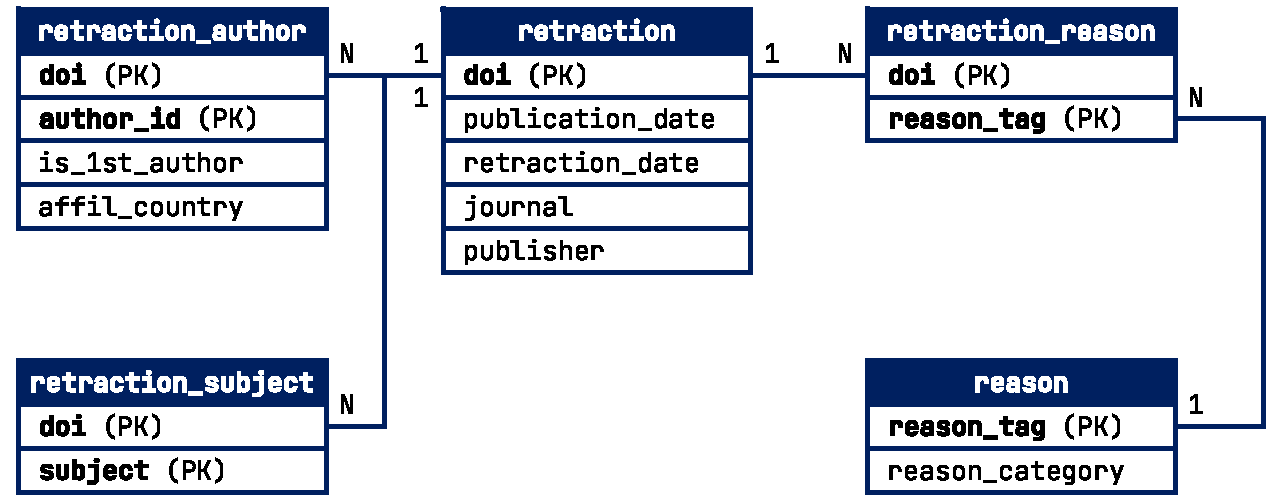
\includegraphics[width=\textwidth]{figures/methods/database-schema.pdf}
    \caption{Lược đồ cơ sở dữ liệu dùng để phân tích ấn phẩm bị thu hồi}
    \label{fig:database-schema}
\end{figure}

Ở bước cuối, dữ liệu sau khi làm sạch, tích hợp và mô hình hóa được xuất dưới định dạng Apache Parquet. Là định dạng lưu trữ theo cột, Parquet phù hợp với các tác vụ phân tích dữ liệu; đồng thời, các nghiên cứu thực nghiệm cho thấy việc chuyển từ CSV sang Parquet có thể giảm kích thước tệp và thời gian xử lý, đồng thời hỗ trợ các kỹ thuật quản lý dữ liệu nâng cao \parencite{fenk2025, bhosale2024}. Do đó, Parquet được lựa chọn làm định dạng lưu trữ cho dữ liệu phân tích của nghiên cứu.

Bên cạnh đó, nghiên cứu sử dụng \textbf{DuckDB} phiên bản 1.3.2 trên nền tảng \textbf{Google Colab} để truy vấn trực tiếp các tệp Parquet bằng SQL, qua đó chỉ khai thác các dòng và cột cần thiết cho từng truy vấn. Các truy vấn SQL được sử dụng để tổng hợp dữ liệu và tạo các bảng đầu ra phục vụ phân tích. Các kết quả này sau đó được trực quan hóa bằng các thư viện {\sffamily matplotlib} và {\sffamily seaborn} trong \textbf{Python} nhằm làm nổi bật các đặc trưng, xu hướng và phát hiện chính. Việc lựa chọn và thiết kế biểu đồ tuân theo các nguyên tắc về xác định bối cảnh, lựa chọn hình thức biểu đồ trực quan phù hợp, giảm yếu tố gây nhiễu và hướng sự chú ý của người đọc theo \cite{knaflic2015}. Đồng thời, các chỉ số và kết quả thống kê mô tả, bao gồm trung bình, trung vị, mode, phân phối dữ liệu và biểu đồ hộp, được tính toán và diễn giải dựa trên \cite{cooksey2020} và \cite{loeb2017}.

Nhìn chung, quy trình đã tích hợp thành công dữ liệu Scopus, WoS với 492 bản ghi từ RWD, đồng thời bảo đảm tính nhất quán, toàn vẹn và khả năng tái lập của dữ liệu sau xử lý. Tập dữ liệu cuối cùng được chuẩn hóa và tổ chức phù hợp cho các phân tích trắc lượng thư mục và diễn giải kết quả tiếp theo.